\pagebreak

\section{User Interface}
The User Interface consists of various components. In this section we will explain their functionality.

\subsection{3D Viewer}
We use \emph{three.js} as a \emph{WebGL} \cite{webgl} abstraction layer. This library is very well tested and makes it extremely easy to manipulate 3D objects. The included  \emph{OrbitControls} \cite{three:orbit-controls} allows for easy camera zooming, rotating and panning.

We will use the \emph{STL Loader} \cite{three:stl-loader}, to load any STL model as a three.js object, as shown in this \href{https://threejs.org/examples/?q=stl#webgl_loader_stl}{demo}.


\autoref{fig:viewer-demo} shows an example of the 3D Viewer with some basic models.

\begin{figure}[H]
    \noindent\makebox[\textwidth]{
        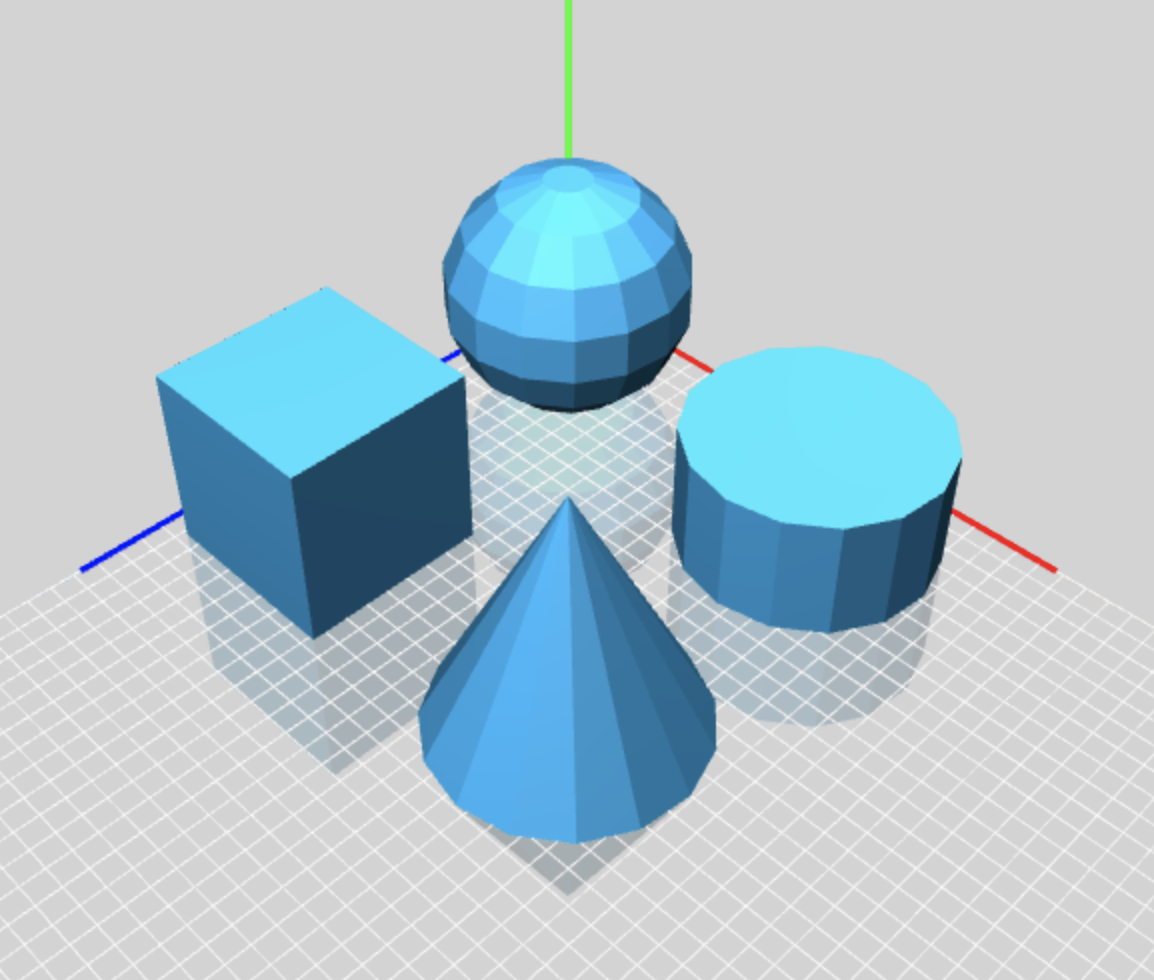
\includegraphics[width=.9\textwidth]{images/models.png}
    }
    \caption{3D Viewer example: Simple objects}
    \label{fig:viewer-demo}
\end{figure}


\subsection{GUI}
We will be using a 2D graphical user interface to allow the user to fine-tune the settings. This is important because of the great variety in 3D printer models that come in different sizes, have different speeds, materials, etc.

This GUI will control both printer-related settings (layer height, speed, temperature, etc), as well as the 3D Viewer settings (object color, rotation, translation, scale, etc).

We choose \emph{dat.GUI} \cite{dat.GUI} for its ease of use, as well as integrated save and load capabilities, that will make it easy to create presets for different printers or qualities. It supports boolean, range and color selectors, as well as actions and folders. This way we can organize the large amount of settings that we need for the project. 

\autoref{fig:dat.GUI} shows an example menu using dat.GUI with some of the settings that we will implement.

\begin{figure}[H]
    \noindent\makebox[\textwidth]{
        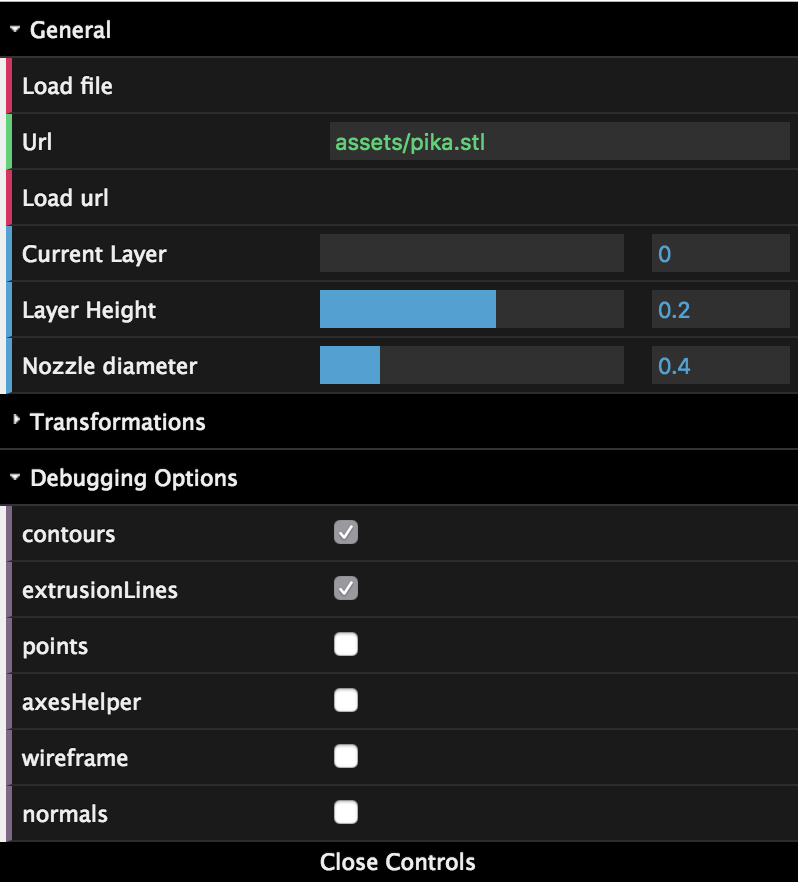
\includegraphics[width=.6\textwidth]{images/datgui.png}
    }
    \caption{dat.GUI: Sample menu}
    \label{fig:dat.GUI}
\end{figure}


Whenever the user changes a setting in the GUI, its \code|onChange()| method is called. dat.GUI also supports data binding, meaning that whenever the user interacts with the settings UI, the corresponding object property will be changed accordingly. We will use this to our advantage to simplify code.

To keep the GUI in the main scope, while keeping access to the data binding features, we will need to have the 3D Viewer communicate with the GUI. We will first create the 3D Viewer, and then pass it as a parameter to the GUI constructor. This ensures the GUI has access to the objects it needs to mutate, while reducing boilerplate code to a minimum. 

There will also be options that are not part of the 3D Viewer. For simplicity, we will be combining all configuration in an object called \code|Config|. This way we can save and restore all user preferences in a simple way.


